\begin{frame}
	\frametitle{Transazioni $\rightarrow$ Blocchi} 
	\framesubtitle{generazione nuova transazione}
	
	\begin{enumerate}
		\item broadcastata nella rete tramite protocollo \textit{flooding}
		\item ogni miner \textbf{può} includerla nel suo \textit{pool}
		\item \textit{invalida} fino a risoluzione del $\mathfrak{B}$ ove viene inserita
		\item a quel punto chi l'ha ancora in pool la rimuove
	\end{enumerate}

	\begin{figure}[H]
		\begin{center}
			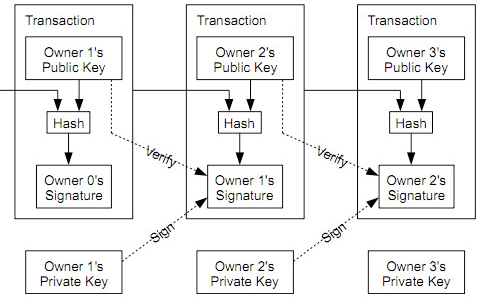
\includegraphics[height = 4.5 cm]{images/chain_transactions.png}	
		\end{center}
	\end{figure}
\end{frame}